\documentclass{article}
\usepackage{graphicx}
\usepackage{hyperref}

\title{BrickGame Tetris Project Documentation}
\author{LIONCOCO}

\begin{document}

\maketitle

\tableofcontents

\section{Introduction}
BrickGame Tetris is a terminal-based version of the classic Tetris game implemented in C using the ncurses library for rendering. The game features block movement, rotation, line clearing, and a scoring system. This documentation provides an overview of the project structure, including the main game logic, user interface, and the installation process.

\section{Game Overview}
In this game, the player controls falling tetrominoes to arrange them in rows. Completed rows are cleared, and the player scores points based on the number of rows cleared at once. The game speeds up as the player progresses through levels, and the game ends when the stack of blocks reaches the top of the playing field.

\section{Project Structure}

\subsection{backend.c and backend.h}
The backend files contain the core logic of the game. This includes:
\begin{itemize}
    \item Spawning new tetrominoes.
    \item Handling tetromino movement (left, right, down) and rotation.
    \item Detecting full lines and clearing them.
    \item Calculating and updating the player's score and level.
\end{itemize}

\subsection{frontend.c and frontend.h}
The frontend files are responsible for rendering the game to the terminal using ncurses. Key components include:
\begin{itemize}
    \item Displaying the game grid and the current tetromino.
    \item Showing the score, level, and next tetromino in the side panel.
    \item Handling user input for controlling the tetromino (e.g., arrow keys for movement and rotation).
\end{itemize}

\subsection{brick\_game.c and brick\_game.h}
This file contains the main game loop, which manages the game state and interaction between the backend and frontend. It handles:
\begin{itemize}
    \item Initializing the game.
    \item Checking for game over conditions.
    \item Transitioning between game states (e.g., active game, pause, game over).
\end{itemize}

\section{Game Flow Diagram}
The game operates as a finite state machine. The following diagram shows the flow of the game states:

\begin{figure}[h]
    \centering
    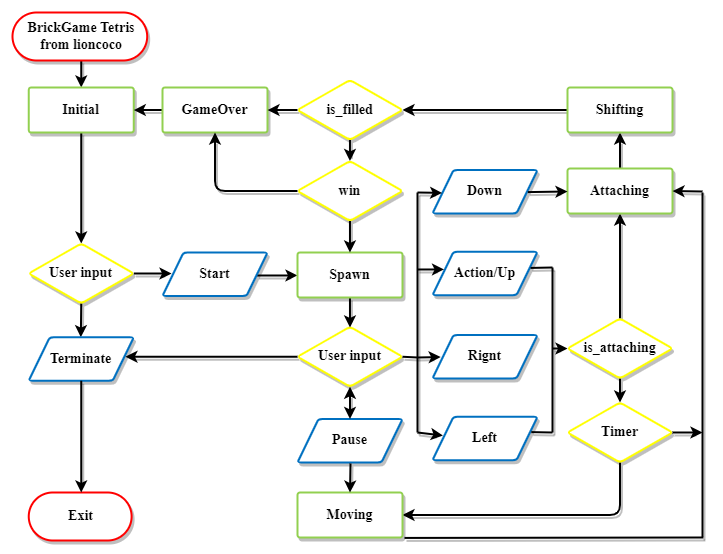
\includegraphics[width=0.8\textwidth]{docs/Diagrama.png}
    \caption{Game Flow Diagram}
    \label{fig:diagram}
\end{figure}

\subsection{State Descriptions}
\begin{itemize}
    \item \textbf{Initial State}: The game is initialized, and the first tetromino spawns.
    \item \textbf{Active State}: The tetromino is falling, and the player can move and rotate it.
    \item \textbf{Line Clear State}: When a full line is completed, it is cleared, and the score is updated.
    \item \textbf{Game Over State}: The game ends when the tetrominoes reach the top of the playing field.
\end{itemize}

\section{Installation}

To install the game, use the following commands:

\begin{verbatim}
make install
\end{verbatim}

The default installation path is stored in the file \texttt{install\_path.txt}, which is set to the default value of `builds'. You can change the installation path by passing a new path during installation:

\begin{verbatim}
make set_install_path
new/path
make install
\end{verbatim}

\section{Gameplay Instructions}
The following keys control the game:
\begin{itemize}
    \item \textbf{Left Arrow}: Move tetromino left.
    \item \textbf{Right Arrow}: Move tetromino right.
    \item \textbf{Up Arrow or Z}: Rotate tetromino.
    \item \textbf{Down Arrow}: Accelerate tetromino fall.
    \item \textbf{Space}: Pause the game.
    \item \textbf{Q or ESC}: Quit the game.
\end{itemize}

\section{Score and Level System}
The player scores points by clearing lines. The points are awarded as follows:
\begin{itemize}
    \item 1 line cleared: 100 points.
    \item 2 lines cleared: 300 points.
    \item 3 lines cleared: 700 points.
    \item 4 lines cleared: 1500 points.
\end{itemize}

Every 600 points increase the level by 1, and the game speeds up. The maximum level is 10.

\section{High Score}
The game keeps track of the highest score achieved, which is saved between sessions. The high score is stored in a file in the installation directory.

\end{document}
